\documentclass[12pt, a4paper]{article}
\usepackage{geometry}
\renewcommand{\baselinestretch}{1.3}
\usepackage[backend = biber, citestyle = authoryear, url = false]{biblatex}
\usepackage{hyperref}
\usepackage{pdflscape}
\usepackage{graphicx}
\addbibresource{sop.bib}
\title{Is small beautiful? Do small districts lead to better outcomes?}
\author{Jothsna Rajan \\
	\small{Indian Institute of Management, Bangalore, India}}
\geometry{a4paper, top=25mm}
\graphicspath{ {Images/} }
\usepackage{Sweave}
\begin{document}
\Sconcordance{concordance:seminar.tex:seminar.Rnw:%
1 13 1 1 0 131 1 1 15 1 1 1 4 44 0 1 3 1 16 40 0 1 23 39 0 1 2 1 13 40 %
0 1 23 39 0 1 2 1 11 15 1 1 16 40 0 1 21 39 0 1 3 1 16 40 0 1 22 39 0 1 %
2 1 15 34 0 1 7 46 0 1 7 46 0 1 7 46 0 1 2 3 5 2 1}

	\maketitle
	\begin{abstract}
		What is the optimal population level at for local public service delivery? In the question over the optimal size of local government systems, small jurisdictions have been attributed a lot of merits. But does bifurcating larger districts into smaller ones pay off? I examine this question in the context of public education using data from a district bifurcation process in Karnataka, India.
	\end{abstract}
\paragraph{} Is there an optimal size for local government systems? Aristotle in his treatise `Politics' argued that political entities needed to balance the twin considerations of economic viability and effective citizenship \parencite{aristotle_politics_1984}. In modern democracies, debates on the topic are framed in a similar language with two sets of normative criteria. The first one is \textit{output legitimacy}. The function of local governments is to provide a set of public goods and services to its citizens and promote public welfare. A government that fulfils this duty better has higher output legitimacy. The other normative concern is `citizen effectiveness' or the capability and willingness of citizens to control the decisions made on their behalf \parencite{dahl_size_1973}. Enhancing citizen effectiveness raises the \textit{input legitimacy} of the system. Both output and input legitimacy are prerequisites to democratic legitimacy \parencite{scharpf_governing_1999}. The fundamental assumption in these debates is that changing the size of political units is likely to affect the democratic quality (input legitimacy) and functional effectiveness (output legitimacy) of governments. There has been attempts to explain the performance of public organizations in terms of the population size that it serves. Recent debates on the topic attribute considerable virtues to small jurisdictions. Holzer et al in 2009 provide a review of the empirical literature in this stream \parencite{holzer2009literature}. 

\paragraph{}  In democratic societies, the economic and political arguments tend to converge. Small jurisdictions are believed to enhance political participation, make politics less abstract, politicians more responsive, and facilitate exit-based empowerment of citizens \parencite{hansen_size_2014}. Decentralisation will also increase economic efficiency as the local governments have an information advantage and can respond better to variance in preferences at the local level \parencite{oates_fiscal_1972}, and population mobility will lead to competition between local authorities and better provision of public goods. Decentralised service delivery especially when citizens directly elect the local governments is expected to provide better coverage, quality and efficiency \parencite{smoke2015rethinking}. Competing local governments may experiment with various ways to provide public goods and lead to innovations that can be applied elsewhere. These considerations suggest that public goods that are (1) sensitive to local preferences and (2) do not have large spillover (3) nor scale effects: infrastructure, public education, etc. are better provided under decentralisation (\cite{tiebout_economies_1960}, \cite{oates_fiscal_1972}).

\paragraph{} In a bid to arrive at the optimal population size in a local government unit, many national governments have opted to create smaller sized local governments. India has seen frequent administrative bifurcations at the local government level (district level). The number of districts in the country has increased from 356 in the 1971 census period to 640 in the 2011 census (Table. \ref{Fig2}) This is a trend that is continuing in the present day. West Bengal has created five new districts since 2015. The rationale for creating of new districts was stated to be - ``...for \textit{better administrative control} and so that \textit{public service can be delivered at the door steps} of the people staying at remote areas'' (emphasis added) \parencite{Mamata}. Similarly, Telangana state is contemplating the creation of 14 - 15 new districts \parencite{Telengana} and Haryana state is considering 3 more districts \parencite{Haryana}. In all these cases, the stated rationale for district bifurcation is decentralisation of administration and better public service. And India is not alone in the implementation of administrative bifurcations at the local government level. Brazil, in the period from 1990 to 2000, increased the number of municipalities from 4,491 to 5,560 \parencite{tomio2005creation}. Russia adopted Local Government Reform in 2003 and since then has doubled the number of municipalities \parencite{turgel2008new}\nocite{avellaneda_is_2015}. Evidence on the effect of size on local government performance is inconclusive  \parencite{holzer2009literature}. Yet, decentralization at the local government level is a step that is frequently taken - despite the lack of empirical examination of its effectiveness. But does creation of new districts enhance public service outcomes?

\paragraph{}There are those who argue that it does not. The critics of decentralisation argue that the its effectiveness is often greatly hampered by the particular context of its implementation. Vito Tanzi offers an argument for corruption to be higher at local levels than at central government levels, because of closer interaction at the local level between the bureaucrats and citizens that can enable nepotism and personal favours \parencite{tanzi1996macroeconomic}. Also, local bureaucracies may be poorly staffed and ill-equipped to handle the responsibilities associated with the decentralised provision of public goods \parencite{prud1995dangers}. The precise nature of decentralisation, such as the financial autonomy of the local government may also pay a role in determining whether the benefits can be reaped. These factors caution against the implementation of decentralisation as a panacea for administrative ills. It also means that any instance of decentralisation can be explored further to understand the context of success or failure.

\paragraph{} There is evidence from the decentralisation reforms in Bolivia and Columbia to suggest that decentralisation has enhanced the local allocative efficiency of public funds. Notably, it has resulted in shifting resources towards education in regions where education performance has historically been worse. But data limitations prevent the authors from testing whether the improvement extends to education outcomes, such as literacy and test scores \parencite{faguet2008decentralization}. Also, there is evidence from California state, to suggest that students in smaller districts perform better than those in larger districts in standardised tests after controlling for a variety of other factors \parencite{driscoll2003school}. The effect of each of these policies - bifurcation or consolidation or a combination of both - depends on the particular context and capabilities of the local administrative body. 

\paragraph{}This paper explores the impact of bifurcation of districts on the quality of public service delivery - specifically, the quality of public education. Public education is not seen as imposing strong externalities on neighbouring regions, nor does it have large scale effects. Therefore, under the classic explanation, a smaller district should be able to provide better service. At the same time, we might need to build administrative capacity when a larger district is split into two or more before any benefits can be reaped. Also, if the districts are too small in the first place, there might be some benefit in consolidating two or more districts and managing them together. I test my propositions using data collected on public education settings in the districts of Karnataka in India over a 9 year period from 2005 to 2013. In the last decade Karnataka state in the south of India carved out three new districts from three existing ones. A new district is created by reallocating some of the taluks (sub-districts) within a district to a new one. Two new districts were created from two existing ones in 2007, and a third new district was created from an existing one in 2010 taking the total in the state up to 30. 
\paragraph{} Creation of a new district entail additional administrative costs as the new districts often need to create the administrative infrastructure. In this paper I estimate the effect of the bifurcation of the administrative district on the public spending and quality of educational service delivered in the district. The identification is complicated by the fact the districts that were not split may be different from those that were. The demand for creation a new district usually arises from within the district, and the political traction gained by the idea has a role to play in the eventual decision made by the state. 

%\section*{Methodology}
Spatial and temporal variation in public policy affords the conditions suitable for identifying the impact of the policy on outcomes. But often the policy is endogenous and can be included in the left \textit{or} right side of the equation. 
\printbibliography
\section*{Appendix}
\begin{table}[h!]
	\centering
	\caption{New Districts created in India - Statewise}
	\label{Fig1}
	\begin{tabular}{c|cccc} 
		\hline
		States/UTs & 1971-81 & 1981-91 & 1991-2001 & 2001-11 \\
		\hline 
		Andaman and Nicobar Islands & 1 & 0 & 0 & 1  \\ 
		Andhra Pradesh & 2 & 0 & 0 & 0  \\ 
		Arunachal Pradesh & 4 & 2 & 2 & 3  \\ 
		Assam & 0 & 13 & 0 & 4  \\ 
		Bihar & 14 & 11 & 8 & 1  \\ 
		Chhattisgarh & 0 & 0 & 9 & 2  \\ 
		Daman and Diu & 0 & 2 & 0 & 0  \\ 
		Delhi & 0 & 0 & 8 & 0  \\ 
		Goa & 0 & -1 & 0 & 0  \\ 
		Gujarat & 0 & 0 & 6 & 1  \\ 
		Haryana & 5 & 4 & 3 & 2  \\ 
		Himachal Pradesh & 2 & 0 & 0 & 0  \\ 
		Jammu and Kashmir & 4 & 0 & 0 & 8  \\ 
		Jharkhand & 0 & 0 & 5 & 6  \\ 
		Karnataka & 0 & 1 & 7 & 3  \\ 
		Kerala & 2 & 2 & 0 & 0  \\ 
		Madhya Pradesh & 2 & 0 & 7 & 5  \\ 
		Maharashtra & 0 & 4 & 5 & 0  \\ 
		Manipur & 1 & 2 & 1 & 0  \\ 
		Meghalaya & 3 & 0 & 2 & 0  \\ 
		Mizoram & 3 & 0 & 5 & 0  \\ 
		Nagaland & 4 & 0 & 1 & 3  \\ 
		Odisha & 0 & 0 & 17 & 0  \\ 
		Punjab & 1 & 0 & 5 & 3  \\ 
		Rajasthan & 0 & 1 & 5 & 1  \\ 
		Tamil Nadu & 2 & 5 & 9 & 2  \\ 
		Tripura & 0 & 0 & 1 & 0  \\ 
		Uttar Pradesh & 2 & 7 & 16 & 1  \\ 
		Uttarakhand & 0 & 0 & 4 & 0  \\ 
		West Bengal & 0 & 1 & 1 & 1  \\ 
		\hline
		Overall & 52 & 54 & 127 & 47  \\ 
		\hline
	\end{tabular}
\end{table}

\begin{table}[h!]
	\centering
	\caption{No\# of Districts in India - Statewise}
	\label{Fig2}
	\begin{tabular}{c|ccccc} 
		\hline
		States/UTs & 1971 & 1981 & 1991 & 2001 & 2011 \\
		\hline 
		Andaman \& Nicobar Islands & 1 & 2 & 2 & 2 & 3 \\ 
		Andhra Pradesh & 21 & 23 & 23 & 23 & 23 \\ 
		Arunachal Pradesh & 5 & 9 & 11 & 13 & 16 \\ 
		Assam & 10 & 10 & 23 & 23 & 27 \\ 
		Bihar & 17 & 31 & 42 & 37 & 38 \\ 
		Chandigarh & 1 & 1 & 1 & 1 & 1 \\ 
		Chhattisgarh &  &  &  & 16 & 18 \\ 
		Dadra \& Nagar Haveli & 1 & 1 & 1 & 1 & 1 \\ 
		Daman \& Diu &  &  & 2 & 2 & 2 \\ 
		Delhi & 1 & 1 & 1 & 9 & 9 \\ 
		Goa & 3 & 3 & 2 & 2 & 2 \\ 
		Gujarat & 19 & 19 & 19 & 25 & 26 \\ 
		Haryana & 7 & 12 & 16 & 19 & 21 \\ 
		Himachal Pradesh & 10 & 12 & 12 & 12 & 12 \\ 
		Jammu \& Kashmir & 10 & 14 & 14 & 14 & 22 \\ 
		Jharkhand &  &  &  & 18 & 24 \\ 
		Karnataka & 19 & 19 & 20 & 27 & 30 \\ 
		Kerala & 10 & 12 & 14 & 14 & 14 \\ 
		Lakshadweep & 1 & 1 & 1 & 1 & 1 \\ 
		Madhya Pradesh & 43 & 45 & 45 & 45 & 50 \\ 
		Maharashtra & 26 & 26 & 30 & 35 & 35 \\ 
		Manipur & 5 & 6 & 8 & 9 & 9 \\ 
		Meghalaya & 2 & 5 & 5 & 7 & 7 \\ 
		Mizoram &  & 3 & 3 & 8 & 8 \\ 
		Nagaland & 3 & 7 & 7 & 8 & 11 \\ 
		Orissa & 13 & 13 & 13 & 30 & 30 \\ 
		Pondicherry & 4 & 4 & 4 & 4 & 4 \\ 
		Punjab & 11 & 12 & 12 & 17 & 20 \\ 
		Rajasthan & 26 & 26 & 27 & 32 & 33 \\ 
		Sikkim & 4 & 4 & 4 & 4 & 4 \\ 
		Tamil Nadu & 14 & 16 & 21 & 30 & 32 \\ 
		Tripura & 3 & 3 & 3 & 4 & 4 \\ 
		Uttar Pradesh & 54 & 56 & 63 & 70 & 71 \\ 
		Uttaranchal &  &  &  & 13 & 13 \\ 
		West Bengal & 16 & 16 & 17 & 18 & 19 \\ 
		\hline
		States & 19 & 22 & 25 & 29 &  \\ 
		Union Territories & 10 & 9 & 7 & 6 &  \\ 
		Districts & 356 & 412 & 466 & 593 & 640 \\ 
		\hline
	\end{tabular}
\end{table}


\begin{landscape}
% Table created by stargazer v.5.2 by Marek Hlavac, Harvard University. E-mail: hlavac at fas.harvard.edu
% Date and time: Mon, Jul 11, 2016 - 12:50:31 AM
\begin{table}[!htbp] \centering 
  \caption{No of Schools District-wise, across the years} 
  \label{} 
\footnotesize 
\begin{tabular}{@{\extracolsep{5pt}} ccccccccccc} 
\\[-1.8ex]\hline 
\hline \\[-1.8ex] 
 & District & Yr2005 & Yr2006 & Yr2007 & Yr2008 & Yr2009 & Yr2010 & Yr2011 & Yr2012 & NA. \\ 
\hline \\[-1.8ex] 
1 & BAGALKOT & $229$ & $255.0$ & $265.0$ & $269.0$ & $277.0$ & $281$ & $340.0$ & $291.0$ & $292.0$ \\ 
2 & BANGALORE RURAL & $330$ & $324.0$ & $330$ & $328.0$ & $332.0$ & $330.0$ & $367.0$ & $340.0$ & $343.0$ \\ 
3 & BELGAUM & $260$ & $277.0$ & $269.0$ & $283$ & $285.0$ & $291.0$ & $366.0$ & $304.0$ & $304.0$ \\ 
4 & BELGAUM CHIKKODI & $337.0$ & $358.0$ & $291$ & $307.0$ & $320.0$ & $324.0$ & $383.0$ & $328.0$ & $332.0$ \\ 
5 & BELLARY & $213.0$ & $224.0$ & $228$ & $231.0$ & $232$ & $240.0$ & $290.0$ & $246.0$ & $244.0$ \\ 
6 & BIDAR & $262.0$ & $290$ & $322.0$ & $336.0$ & $358.0$ & $377.0$ & $471.0$ & $399.0$ & $414.0$ \\ 
7 & BIJAPUR & $326.0$ & $336.0$ & $327$ & $336.0$ & $345$ & $366$ & $439$ & $392.0$ & $396$ \\ 
8 & CHAMARAJANAGARA & $310$ & $254$ & $180$ & $184.0$ & $186$ & $188.0$ & $229.0$ & $189.0$ & $188.0$ \\ 
9 & CHIKKABALLAPURA & $307.0$ & $295.0$ & $300$ & $309.0$ & $312.0$ & $313.0$ & $357$ & $321.0$ & $319.0$ \\ 
10 & CHIKKAMANGALORE & $253.0$ & $261.0$ & $235.0$ & $224.0$ & $218.0$ & $221.0$ & $258$ & $223.0$ & $225.0$ \\ 
11 & CHITRADURGA & $309.0$ & $310.0$ & $315$ & $330.0$ & $332.0$ & $335.0$ & $398$ & $340$ & $342$ \\ 
12 & DAKSHINA KANNADA & $218.0$ & $223.0$ & $226.0$ & $229$ & $231.0$ & $232.0$ & $294.0$ & $234$ & $235.0$ \\ 
13 & DAVANAGERE & $262.0$ & $268.0$ & $274.0$ & $273.0$ & $275.0$ & $278.0$ & $346.0$ & $279.0$ & $282.0$ \\ 
14 & DHARWAD & $197.0$ & $207.0$ & $145$ & $148.0$ & $153.0$ & $149.0$ & $185.0$ & $152$ & $156.0$ \\ 
15 & GADAG & $128.0$ & $131$ & $135.0$ & $135.0$ & $138.0$ & $141.0$ & $183$ & $146$ & $145.0$ \\ 
16 & GULBARGA & $244.0$ & $252.0$ & $262$ & $283$ & $290.0$ & $300.0$ & $365.0$ & $322.0$ & $326.0$ \\ 
17 & HASSAN & $364.0$ & $367$ & $365$ & $367.0$ & $366.0$ & $371.0$ & $428.0$ & $362.0$ & $363.0$ \\ 
18 & HAVERI & $171.0$ & $176.0$ & $180.0$ & $187.0$ & $191.0$ & $195.0$ & $242.0$ & $199.0$ & $200.0$ \\ 
19 & KODAGU & $168$ & $172.0$ & $173.0$ & $178.0$ & $178.0$ & $178.0$ & $226.0$ & $179$ & $181.0$ \\ 
20 & KOLAR & $421$ & $437.0$ & $419$ & $402.0$ & $403.0$ & $405.0$ & $449.0$ & $406.0$ & $404$ \\ 
21 & KOPPAL & $265$ & $271$ & $288$ & $292.0$ & $297.0$ & $305.0$ & $369.0$ & $325.0$ & $334$ \\ 
22 & MANDYA & $294.0$ & $295.0$ & $296.0$ & $298$ & $296.0$ & $298.0$ & $344.0$ & $302.0$ & $292.0$ \\ 
23 & MYSORE & $293.0$ & $301.0$ & $303.0$ & $307.0$ & $310.0$ & $315.0$ & $370$ & $316.0$ & $315.0$ \\ 
24 & RAICHUR & $294.0$ & $308$ & $324.0$ & $348.0$ & $361$ & $381$ & $445.0$ & $394.0$ & $402.0$ \\ 
25 & RAMANAGARA & $388.0$ & $386.0$ & $395.0$ & $396.0$ & $401$ & $406.0$ & $454.0$ & $391.0$ & $392.0$ \\ 
26 & SHIMOGA & $319.0$ & $317.0$ & $327.0$ & $329.0$ & $331.0$ & $333.0$ & $389.0$ & $335.0$ & $332$ \\ 
27 & TUMKUR & $436$ & $436$ & $445.0$ & $435.0$ & $436.0$ & $429$ & $496.0$ & $427.0$ & $423.0$ \\ 
28 & TUMKUR MADHUGIRI & $351$ & $346$ & $352.0$ & $352.0$ & $358.0$ & $362.0$ & $422$ & $363.0$ & $364.0$ \\ 
29 & UDUPI & $284.0$ & $283$ & $200$ & $192.0$ & $194.0$ & $194.0$ & $258.0$ & $196.0$ & $196.0$ \\ 
30 & UTTARA KANNADA & $212.0$ & $216.0$ & $215.0$ & $219.0$ & $219.0$ & $219.0$ & $249$ & $221.0$ & $221.0$ \\ 
31 & UTTARA KANNADA SIRSI & $200.0$ & $200.0$ & $203$ & $208$ & $209$ & $207.0$ & $234.0$ & $209$ & $209.0$ \\ 
32 & YADAGIRI & $298.0$ & $311.0$ & $328.0$ & $339.0$ & $358$ & $374.0$ & $441.0$ & $398$ & $404$ \\ 
\hline \\[-1.8ex] 
\end{tabular} 
\end{table} \end{landscape}
% Table created by stargazer v.5.2 by Marek Hlavac, Harvard University. E-mail: hlavac at fas.harvard.edu
% Date and time: Mon, Jul 11, 2016 - 12:50:31 AM
\begin{table}[!htbp] \centering 
  \caption{Summary Statistics in 2005} 
  \label{} 
\begin{tabular}{@{\extracolsep{5pt}} ccc} 
\\[-1.8ex]\hline 
\hline \\[-1.8ex] 
 & Undivided & Divided \\ 
\hline \\[-1.8ex] 
TotalMarks & $321.0$ & $302.0$ \\ 
Rural & $0.9$ & $0.9$ \\ 
WorkDays & $89.0$ & $102.0$ \\ 
AcadInsp & $0.5$ & $0.4$ \\ 
DevGrantR & $2,765.0$ & $2,592.0$ \\ 
DevGrantE & $1,641.0$ & $1,298.0$ \\ 
TLMGrantR & $3,537.0$ & $3,989.0$ \\ 
TLMGrantE & $1,763.0$ & $1,793.0$ \\ 
Classrooms & $4.0$ & $3.4$ \\ 
ToiletG & $1$ & $1$ \\ 
Electricity & $0.7$ & $0.5$ \\ 
Library & $0.8$ & $0.8$ \\ 
PlayGround & $0.6$ & $0.5$ \\ 
Male\_Tch & $2.4$ & $2.0$ \\ 
Female\_Tch & $2.0$ & $1.6$ \\ 
Grad\_Tch & $30.0$ & $26.0$ \\ 
ProfQ\_Tch & $4.2$ & $3.3$ \\ 
Days\_nonTch & $0.8$ & $1.9$ \\ 
Public & $0.9$ & $0.9$ \\ 
Split & $0$ & $1$ \\ 
Households & $49,571.0$ & $47,044.0$ \\ 
TotPop & $256,392.0$ & $247,430.0$ \\ 
Pop0.6 & $35,845.0$ & $36,113.0$ \\ 
Literates & $138,828.0$ & $120,988.0$ \\ 
TotWPop & $116,550.0$ & $117,529.0$ \\ 
SCST & $63,916.0$ & $75,581.0$ \\ 
Yr2005 & $276.0$ & $333.0$ \\ 
SchoolperPop2005 & $1.2$ & $1.4$ \\ 
\hline \\[-1.8ex] 
\multicolumn{3}{l}{Population figures used to calculate SchoolperPop2005 is from 2001} \\ 
\end{tabular} 
\end{table} % Table created by stargazer v.5.2 by Marek Hlavac, Harvard University. E-mail: hlavac at fas.harvard.edu
% Date and time: Mon, Jul 11, 2016 - 12:50:32 AM
\begin{table}[!htbp] \centering 
  \caption{Summary Statistics in 2005} 
  \label{} 
\begin{tabular}{@{\extracolsep{5pt}} ccc} 
\\[-1.8ex]\hline 
\hline \\[-1.8ex] 
 & Old & New \\ 
\hline \\[-1.8ex] 
TotalMarks & $295.0$ & $310.0$ \\ 
Rural & $0.9$ & $0.9$ \\ 
WorkDays & $102.0$ & $102.0$ \\ 
AcadInsp & $0.5$ & $0.3$ \\ 
DevGrantR & $2,554.0$ & $2,640.0$ \\ 
DevGrantE & $1,290.0$ & $1,309.0$ \\ 
TLMGrantR & $4,093.0$ & $3,857.0$ \\ 
TLMGrantE & $1,872.0$ & $1,691.0$ \\ 
Classrooms & $3.6$ & $3.3$ \\ 
ToiletG & $1$ & $1$ \\ 
Electricity & $0.5$ & $0.5$ \\ 
Library & $0.8$ & $0.7$ \\ 
PlayGround & $0.5$ & $0.5$ \\ 
Male\_Tch & $2.0$ & $2.0$ \\ 
Female\_Tch & $1.8$ & $1.4$ \\ 
Grad\_Tch & $26.0$ & $26.0$ \\ 
ProfQ\_Tch & $3.5$ & $3.0$ \\ 
Days\_nonTch & $1.5$ & $2.5$ \\ 
Public & $0.9$ & $0.9$ \\ 
Split & $1$ & $1$ \\ 
Households & $47,435.0$ & $46,546$ \\ 
TotPop & $252,924.0$ & $240,438.0$ \\ 
Pop0.6 & $36,703.0$ & $35,362.0$ \\ 
Literates & $131,616.0$ & $107,461.0$ \\ 
TotWPop & $115,871.0$ & $119,639$ \\ 
SCST & $75,410.0$ & $75,798.0$ \\ 
Yr2005 & $333.0$ & $333.0$ \\ 
SchoolperPop2005 & $1.4$ & $1.5$ \\ 
New & $0$ & $1$ \\ 
\hline \\[-1.8ex] 
\multicolumn{3}{l}{Population figures used to calculate SchoolperPop2005 is from 2001} \\ 
\end{tabular} 
\end{table} 
% Table created by stargazer v.5.2 by Marek Hlavac, Harvard University. E-mail: hlavac at fas.harvard.edu
% Date and time: Mon, Jul 11, 2016 - 12:50:32 AM
\begin{table}[!htbp] \centering 
  \caption{Summary Statistics in 2013} 
  \label{} 
\begin{tabular}{@{\extracolsep{5pt}} ccc} 
\\[-1.8ex]\hline 
\hline \\[-1.8ex] 
 & Undivided & Divided \\ 
\hline \\[-1.8ex] 
TotalMarks & $344.0$ & $337.0$ \\ 
Rural & $0.9$ & $0.9$ \\ 
WorkDays & $0.7$ & $0.8$ \\ 
AcadInsp & $1.6$ & $1.3$ \\ 
DevGrantR & $8,657.0$ & $7,328.0$ \\ 
DevGrantE & $7,627.0$ & $6,429.0$ \\ 
TLMGrantR & $1,730.0$ & $1,255.0$ \\ 
TLMGrantE & $1,612.0$ & $1,157.0$ \\ 
Classrooms & $5.3$ & $4.7$ \\ 
ToiletG & $1.0$ & $1.0$ \\ 
Electricity & $1.0$ & $1.0$ \\ 
Library & $1.0$ & $1.1$ \\ 
PlayGround & $0.6$ & $0.5$ \\ 
Male\_Tch & $2.3$ & $2.0$ \\ 
Female\_Tch & $2.4$ & $2.1$ \\ 
Grad\_Tch & $1.0$ & $0.9$ \\ 
ProfQ\_Tch & $4.6$ & $4.0$ \\ 
Days\_nonTch & $0.3$ & $0.3$ \\ 
Public & $0.9$ & $0.8$ \\ 
Split & $0$ & $1$ \\ 
Households & $45,257.0$ & $45,717.0$ \\ 
TotPop & $213,545.0$ & $221,695.0$ \\ 
Pop0.6 & $25,976.0$ & $27,859.0$ \\ 
Literates & $129,884.0$ & $121,608.0$ \\ 
TotWPop & $104,540.0$ & $110,617.0$ \\ 
SCST & $61,425.0$ & $75,293.0$ \\ 
Yr2013 & $291.0$ & $361.0$ \\ 
SchoolperPop2013 & $1.5$ & $1.7$ \\ 
\hline \\[-1.8ex] 
\multicolumn{3}{l}{Population figures used to calculate SchoolperPop2013 is from 2001} \\ 
\end{tabular} 
\end{table} % Table created by stargazer v.5.2 by Marek Hlavac, Harvard University. E-mail: hlavac at fas.harvard.edu
% Date and time: Mon, Jul 11, 2016 - 12:50:32 AM
\begin{table}[!htbp] \centering 
  \caption{Summary Statistics in 2013} 
  \label{} 
\begin{tabular}{@{\extracolsep{5pt}} ccc} 
\\[-1.8ex]\hline 
\hline \\[-1.8ex] 
 & Old & New \\ 
\hline \\[-1.8ex] 
TotalMarks & $342.0$ & $332.0$ \\ 
Rural & $0.9$ & $0.9$ \\ 
WorkDays & $0.7$ & $1.0$ \\ 
AcadInsp & $1.3$ & $1.4$ \\ 
DevGrantR & $7,354.0$ & $7,291.0$ \\ 
DevGrantE & $6,527.0$ & $6,295.0$ \\ 
TLMGrantR & $1,159.0$ & $1,386.0$ \\ 
TLMGrantE & $1,057.0$ & $1,293.0$ \\ 
Classrooms & $4.9$ & $4.4$ \\ 
ToiletG & $1.0$ & $1.0$ \\ 
Electricity & $1.0$ & $1.0$ \\ 
Library & $1.0$ & $1.2$ \\ 
PlayGround & $0.5$ & $0.5$ \\ 
Male\_Tch & $2.1$ & $2.0$ \\ 
Female\_Tch & $2.4$ & $1.8$ \\ 
Grad\_Tch & $1.0$ & $0.8$ \\ 
ProfQ\_Tch & $4.3$ & $3.6$ \\ 
Days\_nonTch & $0.4$ & $0.1$ \\ 
Public & $0.8$ & $0.9$ \\ 
Split & $1$ & $1$ \\ 
Households & $44,657.0$ & $47,163.0$ \\ 
TotPop & $219,607.0$ & $224,543$ \\ 
Pop0.6 & $27,680.0$ & $28,102.0$ \\ 
Literates & $126,225.0$ & $115,311.0$ \\ 
TotWPop & $106,832.0$ & $115,779.0$ \\ 
SCST & $72,394.0$ & $79,247.0$ \\ 
Yr2013 & $357.0$ & $367.0$ \\ 
SchoolperPop2013 & $1.7$ & $1.8$ \\ 
New & $0$ & $1$ \\ 
\hline \\[-1.8ex] 
\multicolumn{3}{l}{Population figures used to calculate SchoolperPop2013 is from 2001} \\ 
\end{tabular} 
\end{table} 
\clearpage
\pagebreak
\begin{figure}[h]
    \centering
    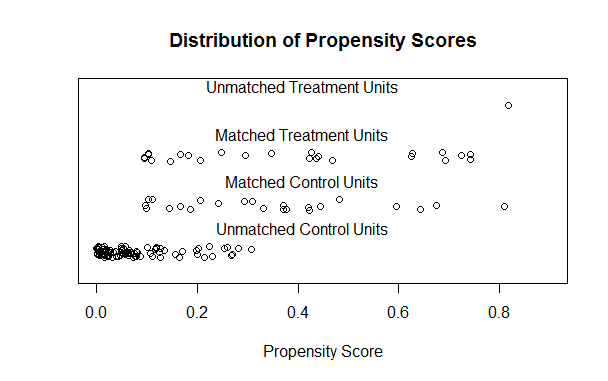
\includegraphics{Jitter}
    \caption{Propensity Score Matching: Jitter Plot}
    \label{Fig1}
\end{figure}

\begin{figure}[h]
    \centering
    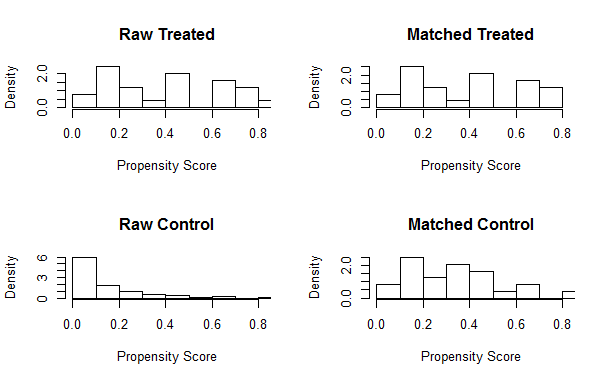
\includegraphics{PSMatch}
    \caption{Propensity Score Matching: Histogram}
    \label{Fig2}
\end{figure}

% Table created by stargazer v.5.2 by Marek Hlavac, Harvard University. E-mail: hlavac at fas.harvard.edu
% Date and time: Mon, Jul 11, 2016 - 12:50:32 AM
\begin{table}[!htbp] \centering 
  \caption{Summary Statistics in 2005 - With PS Matched Control Group} 
  \label{} 
\begin{tabular}{@{\extracolsep{5pt}} ccc} 
\\[-1.8ex]\hline 
\hline \\[-1.8ex] 
 & Undivided & Divided \\ 
\hline \\[-1.8ex] 
TotalMarks & $308.0$ & $302.0$ \\ 
Rural & $0.9$ & $0.9$ \\ 
WorkDays & $90.0$ & $102.0$ \\ 
AcadInsp & $0.5$ & $0.4$ \\ 
DevGrantR & $2,659.0$ & $2,608.0$ \\ 
DevGrantE & $1,470.0$ & $1,279.0$ \\ 
TLMGrantR & $3,585.0$ & $4,007.0$ \\ 
TLMGrantE & $1,966.0$ & $1,777.0$ \\ 
Classrooms & $3.7$ & $3.5$ \\ 
ToiletG & $1$ & $1$ \\ 
Electricity & $0.6$ & $0.5$ \\ 
Library & $0.8$ & $0.8$ \\ 
PlayGround & $0.5$ & $0.5$ \\ 
Male\_Tch & $2.3$ & $2.0$ \\ 
Female\_Tch & $1.7$ & $1.7$ \\ 
Grad\_Tch & $26.0$ & $26.0$ \\ 
ProfQ\_Tch & $3.8$ & $3.3$ \\ 
Days\_nonTch & $1.5$ & $1.8$ \\ 
Public & $0.9$ & $0.9$ \\ 
Split & $0$ & $1$ \\ 
Households & $42,187.0$ & $47,476.0$ \\ 
TotPop & $220,056.0$ & $250,669.0$ \\ 
Pop0.6 & $31,895.0$ & $36,710.0$ \\ 
Literates & $111,360.0$ & $122,912.0$ \\ 
TotWPop & $101,262.0$ & $118,593.0$ \\ 
SCST & $66,376.0$ & $75,755.0$ \\ 
Yr2005 & $299.0$ & $332.0$ \\ 
SchoolperPop2005 & $1.5$ & $1.4$ \\ 
\hline \\[-1.8ex] 
\multicolumn{3}{l}{Population figures used to calculate SchoolperPop2005 is from 2001} \\ 
\end{tabular} 
\end{table} % Table created by stargazer v.5.2 by Marek Hlavac, Harvard University. E-mail: hlavac at fas.harvard.edu
% Date and time: Mon, Jul 11, 2016 - 12:50:32 AM
\begin{table}[!htbp] \centering 
  \caption{Summary Statistics in 2005 - With PS Matched Control Group} 
  \label{} 
\begin{tabular}{@{\extracolsep{5pt}} ccc} 
\\[-1.8ex]\hline 
\hline \\[-1.8ex] 
 & Old & New \\ 
\hline \\[-1.8ex] 
TotalMarks & $295.0$ & $311.0$ \\ 
Rural & $0.9$ & $0.9$ \\ 
WorkDays & $102.0$ & $101.0$ \\ 
AcadInsp & $0.5$ & $0.3$ \\ 
DevGrantR & $2,554.0$ & $2,684.0$ \\ 
DevGrantE & $1,290.0$ & $1,263.0$ \\ 
TLMGrantR & $4,093.0$ & $3,888.0$ \\ 
TLMGrantE & $1,872.0$ & $1,644.0$ \\ 
Classrooms & $3.6$ & $3.3$ \\ 
ToiletG & $1$ & $1$ \\ 
Electricity & $0.5$ & $0.5$ \\ 
Library & $0.8$ & $0.7$ \\ 
PlayGround & $0.5$ & $0.5$ \\ 
Male\_Tch & $2.0$ & $2.0$ \\ 
Female\_Tch & $1.8$ & $1.4$ \\ 
Grad\_Tch & $26.0$ & $26.0$ \\ 
ProfQ\_Tch & $3.5$ & $3.1$ \\ 
Days\_nonTch & $1.5$ & $2.3$ \\ 
Public & $0.9$ & $0.9$ \\ 
Split & $1$ & $1$ \\ 
Households & $47,435.0$ & $47,534.0$ \\ 
TotPop & $252,924.0$ & $247,512.0$ \\ 
Pop0.6 & $36,703.0$ & $36,719.0$ \\ 
Literates & $131,616.0$ & $110,726.0$ \\ 
TotWPop & $115,871.0$ & $122,404.0$ \\ 
SCST & $75,410.0$ & $76,238.0$ \\ 
Yr2005 & $333.0$ & $332.0$ \\ 
SchoolperPop2005 & $1.4$ & $1.5$ \\ 
New & $0$ & $1$ \\ 
\hline \\[-1.8ex] 
\multicolumn{3}{l}{Population figures used to calculate SchoolperPop2005 is from 2001} \\ 
\end{tabular} 
\end{table} 
% Table created by stargazer v.5.2 by Marek Hlavac, Harvard University. E-mail: hlavac at fas.harvard.edu
% Date and time: Mon, Jul 11, 2016 - 12:50:32 AM
\begin{table}[!htbp] \centering 
  \caption{Summary Statistics in 2013 - With PS Matched Control Group} 
  \label{} 
\begin{tabular}{@{\extracolsep{5pt}} ccc} 
\\[-1.8ex]\hline 
\hline \\[-1.8ex] 
 & Undivided & Divided \\ 
\hline \\[-1.8ex] 
TotalMarks & $333.0$ & $340.0$ \\ 
Rural & $0.9$ & $0.9$ \\ 
WorkDays & $0.7$ & $0.9$ \\ 
AcadInsp & $1.4$ & $1.4$ \\ 
DevGrantR & $8,057.0$ & $7,383.0$ \\ 
DevGrantE & $7,440.0$ & $6,503.0$ \\ 
TLMGrantR & $1,427.0$ & $1,238.0$ \\ 
TLMGrantE & $1,384.0$ & $1,148.0$ \\ 
Classrooms & $4.8$ & $4.7$ \\ 
ToiletG & $1.0$ & $1.0$ \\ 
Electricity & $1.0$ & $1.0$ \\ 
Library & $1.0$ & $1.1$ \\ 
PlayGround & $0.6$ & $0.6$ \\ 
Male\_Tch & $2.1$ & $2.1$ \\ 
Female\_Tch & $2.0$ & $2.1$ \\ 
Grad\_Tch & $0.9$ & $0.9$ \\ 
ProfQ\_Tch & $4.1$ & $4.1$ \\ 
Days\_nonTch & $0.2$ & $0.3$ \\ 
Public & $0.9$ & $0.8$ \\ 
Split & $0$ & $1$ \\ 
Households & $44,302.0$ & $46,508.0$ \\ 
TotPop & $209,137.0$ & $227,783.0$ \\ 
Pop0.6 & $25,456.0$ & $28,933.0$ \\ 
Literates & $123,107.0$ & $125,461.0$ \\ 
TotWPop & $103,334.0$ & $113,280.0$ \\ 
SCST & $72,192.0$ & $77,860.0$ \\ 
Yr2013 & $318.0$ & $367.0$ \\ 
SchoolperPop2013 & $1.7$ & $1.7$ \\ 
\hline \\[-1.8ex] 
\multicolumn{3}{l}{Population figures used to calculate SchoolperPop2013 is from 2001} \\ 
\end{tabular} 
\end{table} % Table created by stargazer v.5.2 by Marek Hlavac, Harvard University. E-mail: hlavac at fas.harvard.edu
% Date and time: Mon, Jul 11, 2016 - 12:50:32 AM
\begin{table}[!htbp] \centering 
  \caption{Summary Statistics in 2013 - With PS Matched Control Group} 
  \label{} 
\begin{tabular}{@{\extracolsep{5pt}} ccc} 
\\[-1.8ex]\hline 
\hline \\[-1.8ex] 
 & Old & New \\ 
\hline \\[-1.8ex] 
TotalMarks & $344.0$ & $333.0$ \\ 
Rural & $0.9$ & $0.9$ \\ 
WorkDays & $0.7$ & $1.1$ \\ 
AcadInsp & $1.3$ & $1.6$ \\ 
DevGrantR & $7,260.0$ & $7,574.0$ \\ 
DevGrantE & $6,542.0$ & $6,442.0$ \\ 
TLMGrantR & $1,098.0$ & $1,456.0$ \\ 
TLMGrantE & $1,017.0$ & $1,352.0$ \\ 
Classrooms & $4.9$ & $4.5$ \\ 
ToiletG & $1.0$ & $1.0$ \\ 
Electricity & $1.0$ & $1.0$ \\ 
Library & $1.0$ & $1.2$ \\ 
PlayGround & $0.6$ & $0.5$ \\ 
Male\_Tch & $2.1$ & $2.1$ \\ 
Female\_Tch & $2.4$ & $1.8$ \\ 
Grad\_Tch & $1.0$ & $0.7$ \\ 
ProfQ\_Tch & $4.4$ & $3.7$ \\ 
Days\_nonTch & $0.5$ & $0.1$ \\ 
Public & $0.8$ & $0.9$ \\ 
Split & $1$ & $1$ \\ 
Households & $45,379.0$ & $48,264.0$ \\ 
TotPop & $222,491.0$ & $236,014.0$ \\ 
Pop0.6 & $27,863.0$ & $30,597.0$ \\ 
Literates & $129,369.0$ & $119,382.0$ \\ 
TotWPop & $108,226$ & $121,141$ \\ 
SCST & $73,461.0$ & $84,702$ \\ 
Yr2013 & $362.0$ & $375.0$ \\ 
SchoolperPop2013 & $1.7$ & $1.8$ \\ 
New & $0$ & $1$ \\ 
\hline \\[-1.8ex] 
\multicolumn{3}{l}{Population figures used to calculate SchoolperPop2013 is from 2001} \\ 
\end{tabular} 
\end{table} 



\end{document}
